\appendix

\chapter{Anexo}
\section{Ensayos de movimiento}

\begin{figure}	
	\begin{minipage}{\linewidth}
		\centering
		\subfloat[$X_2 = 60 - 10 = 50\,\mathrm{mm}$]{
			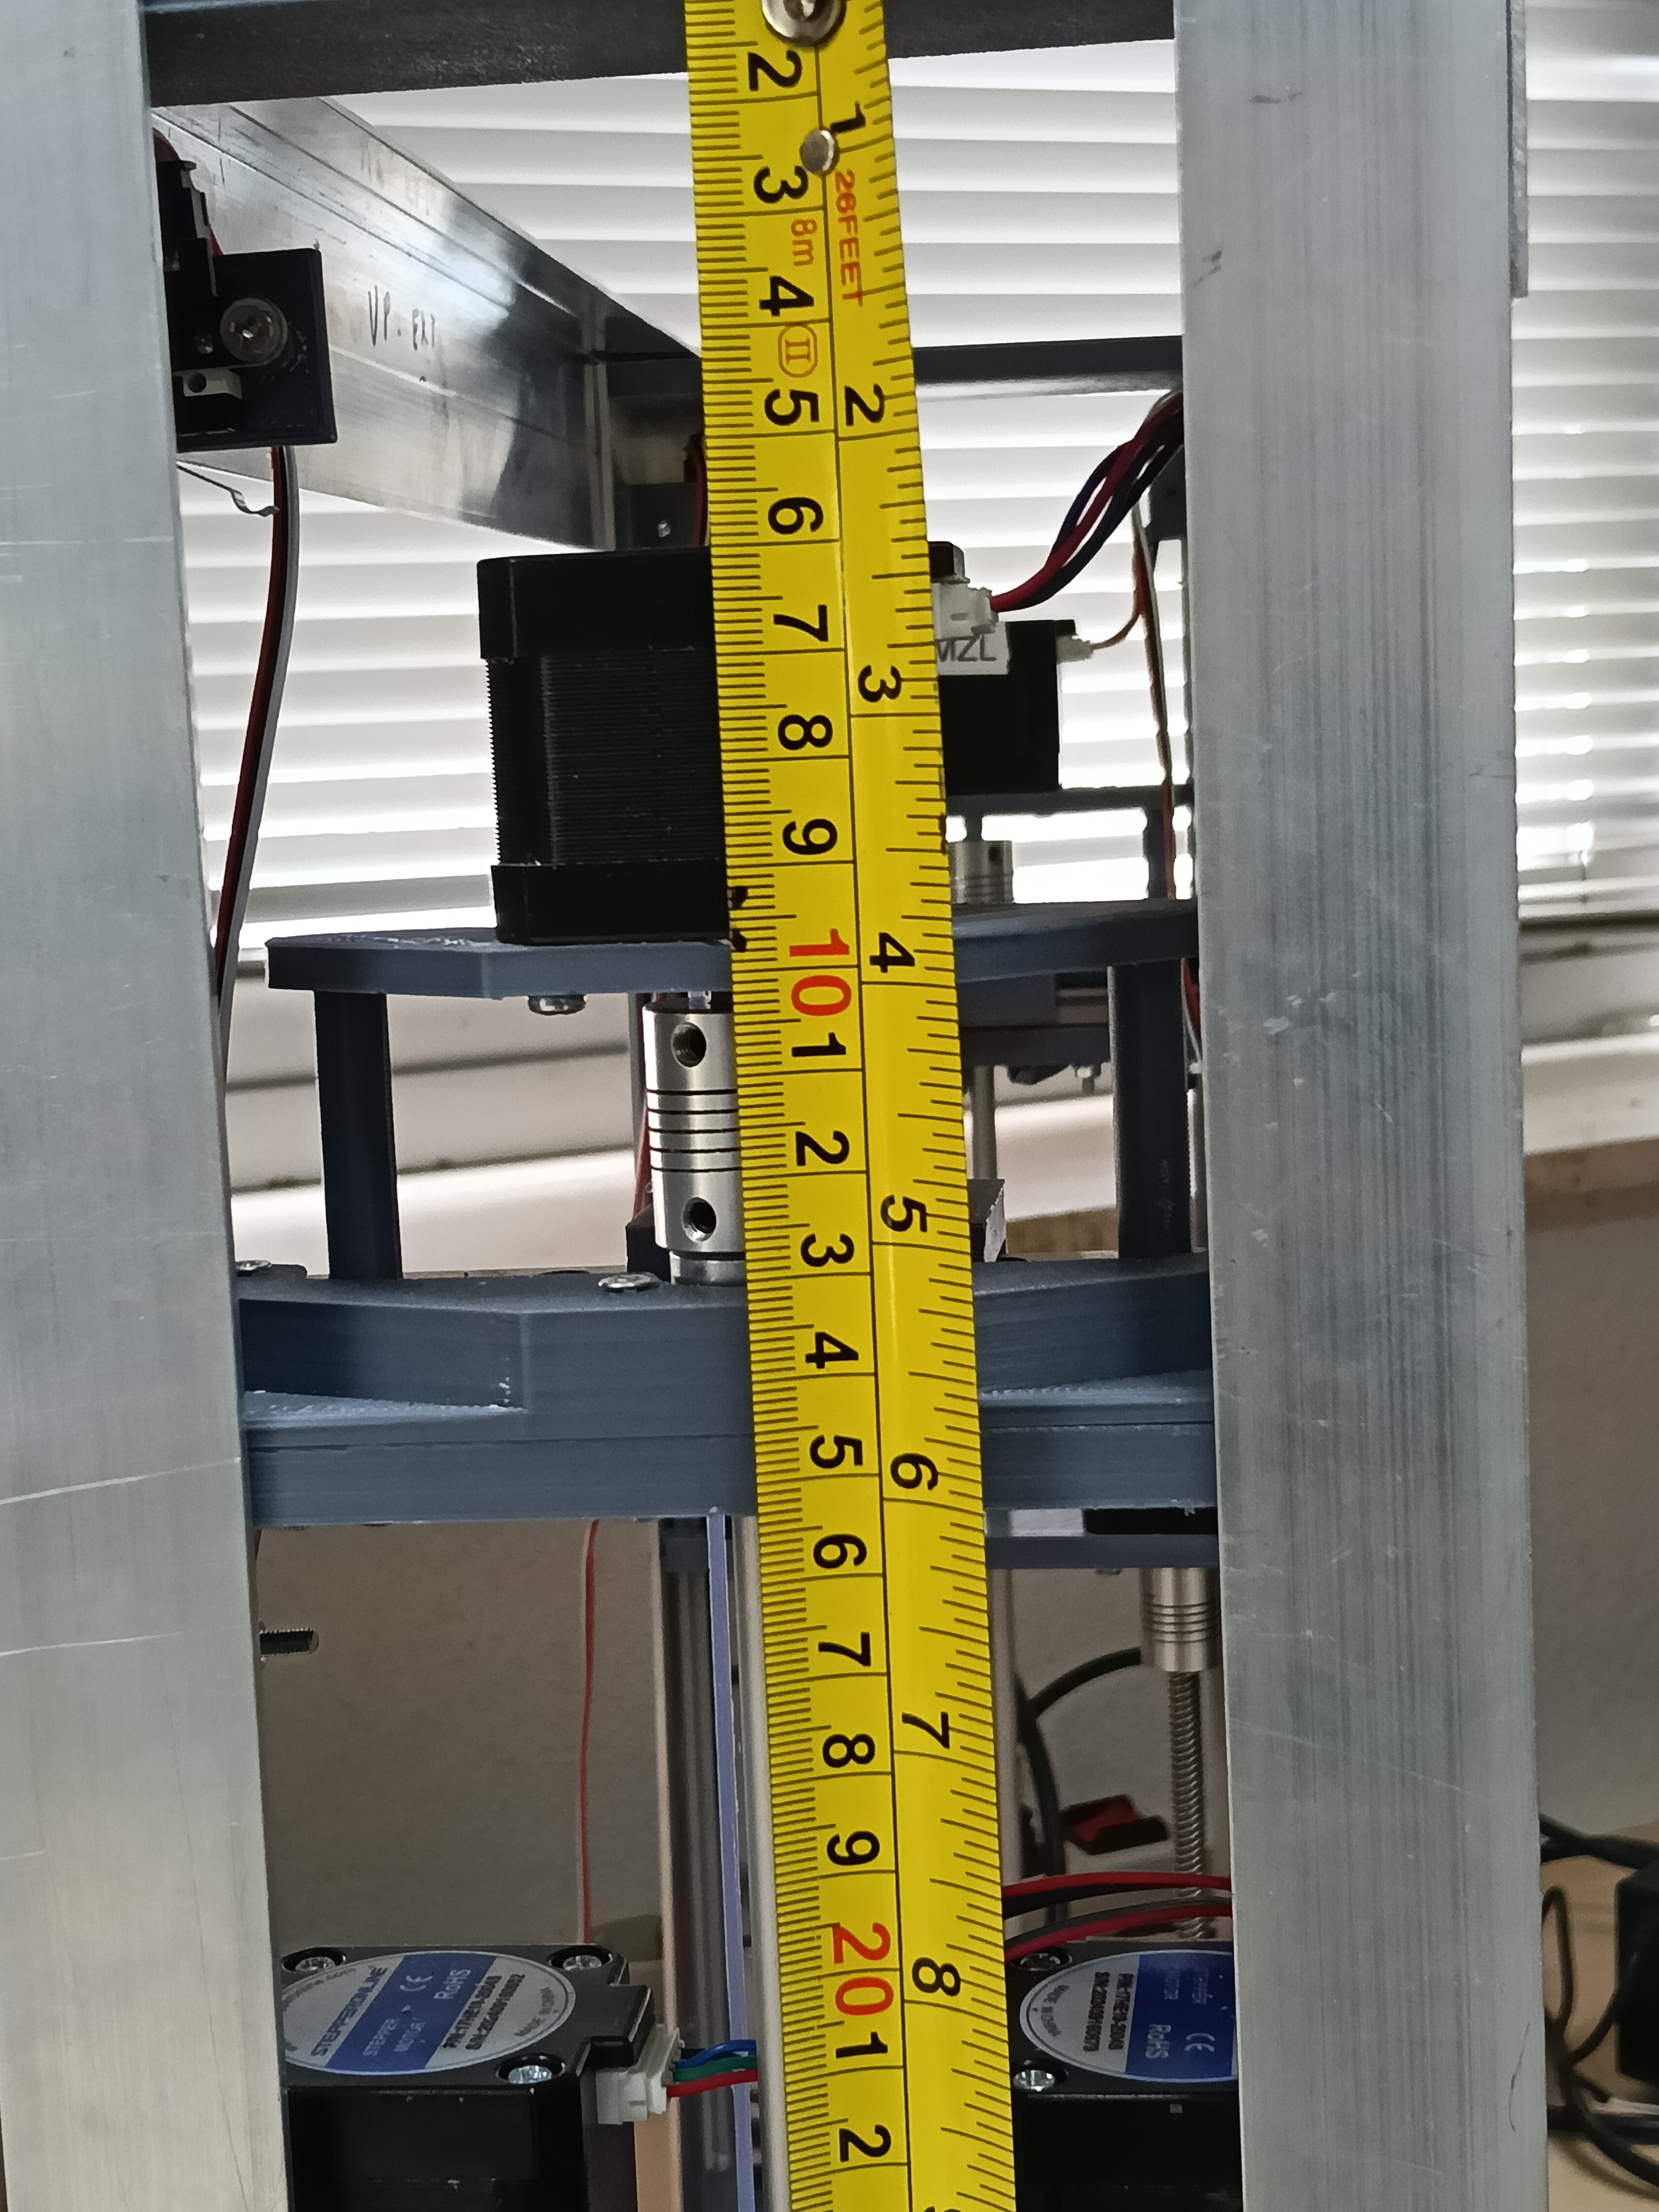
\includegraphics[width=0.45\linewidth]{figuras/pmmvb}
		}
		\subfloat[$Z_2 = 85 - 35 = 50\,\mathrm{mm}$]{
			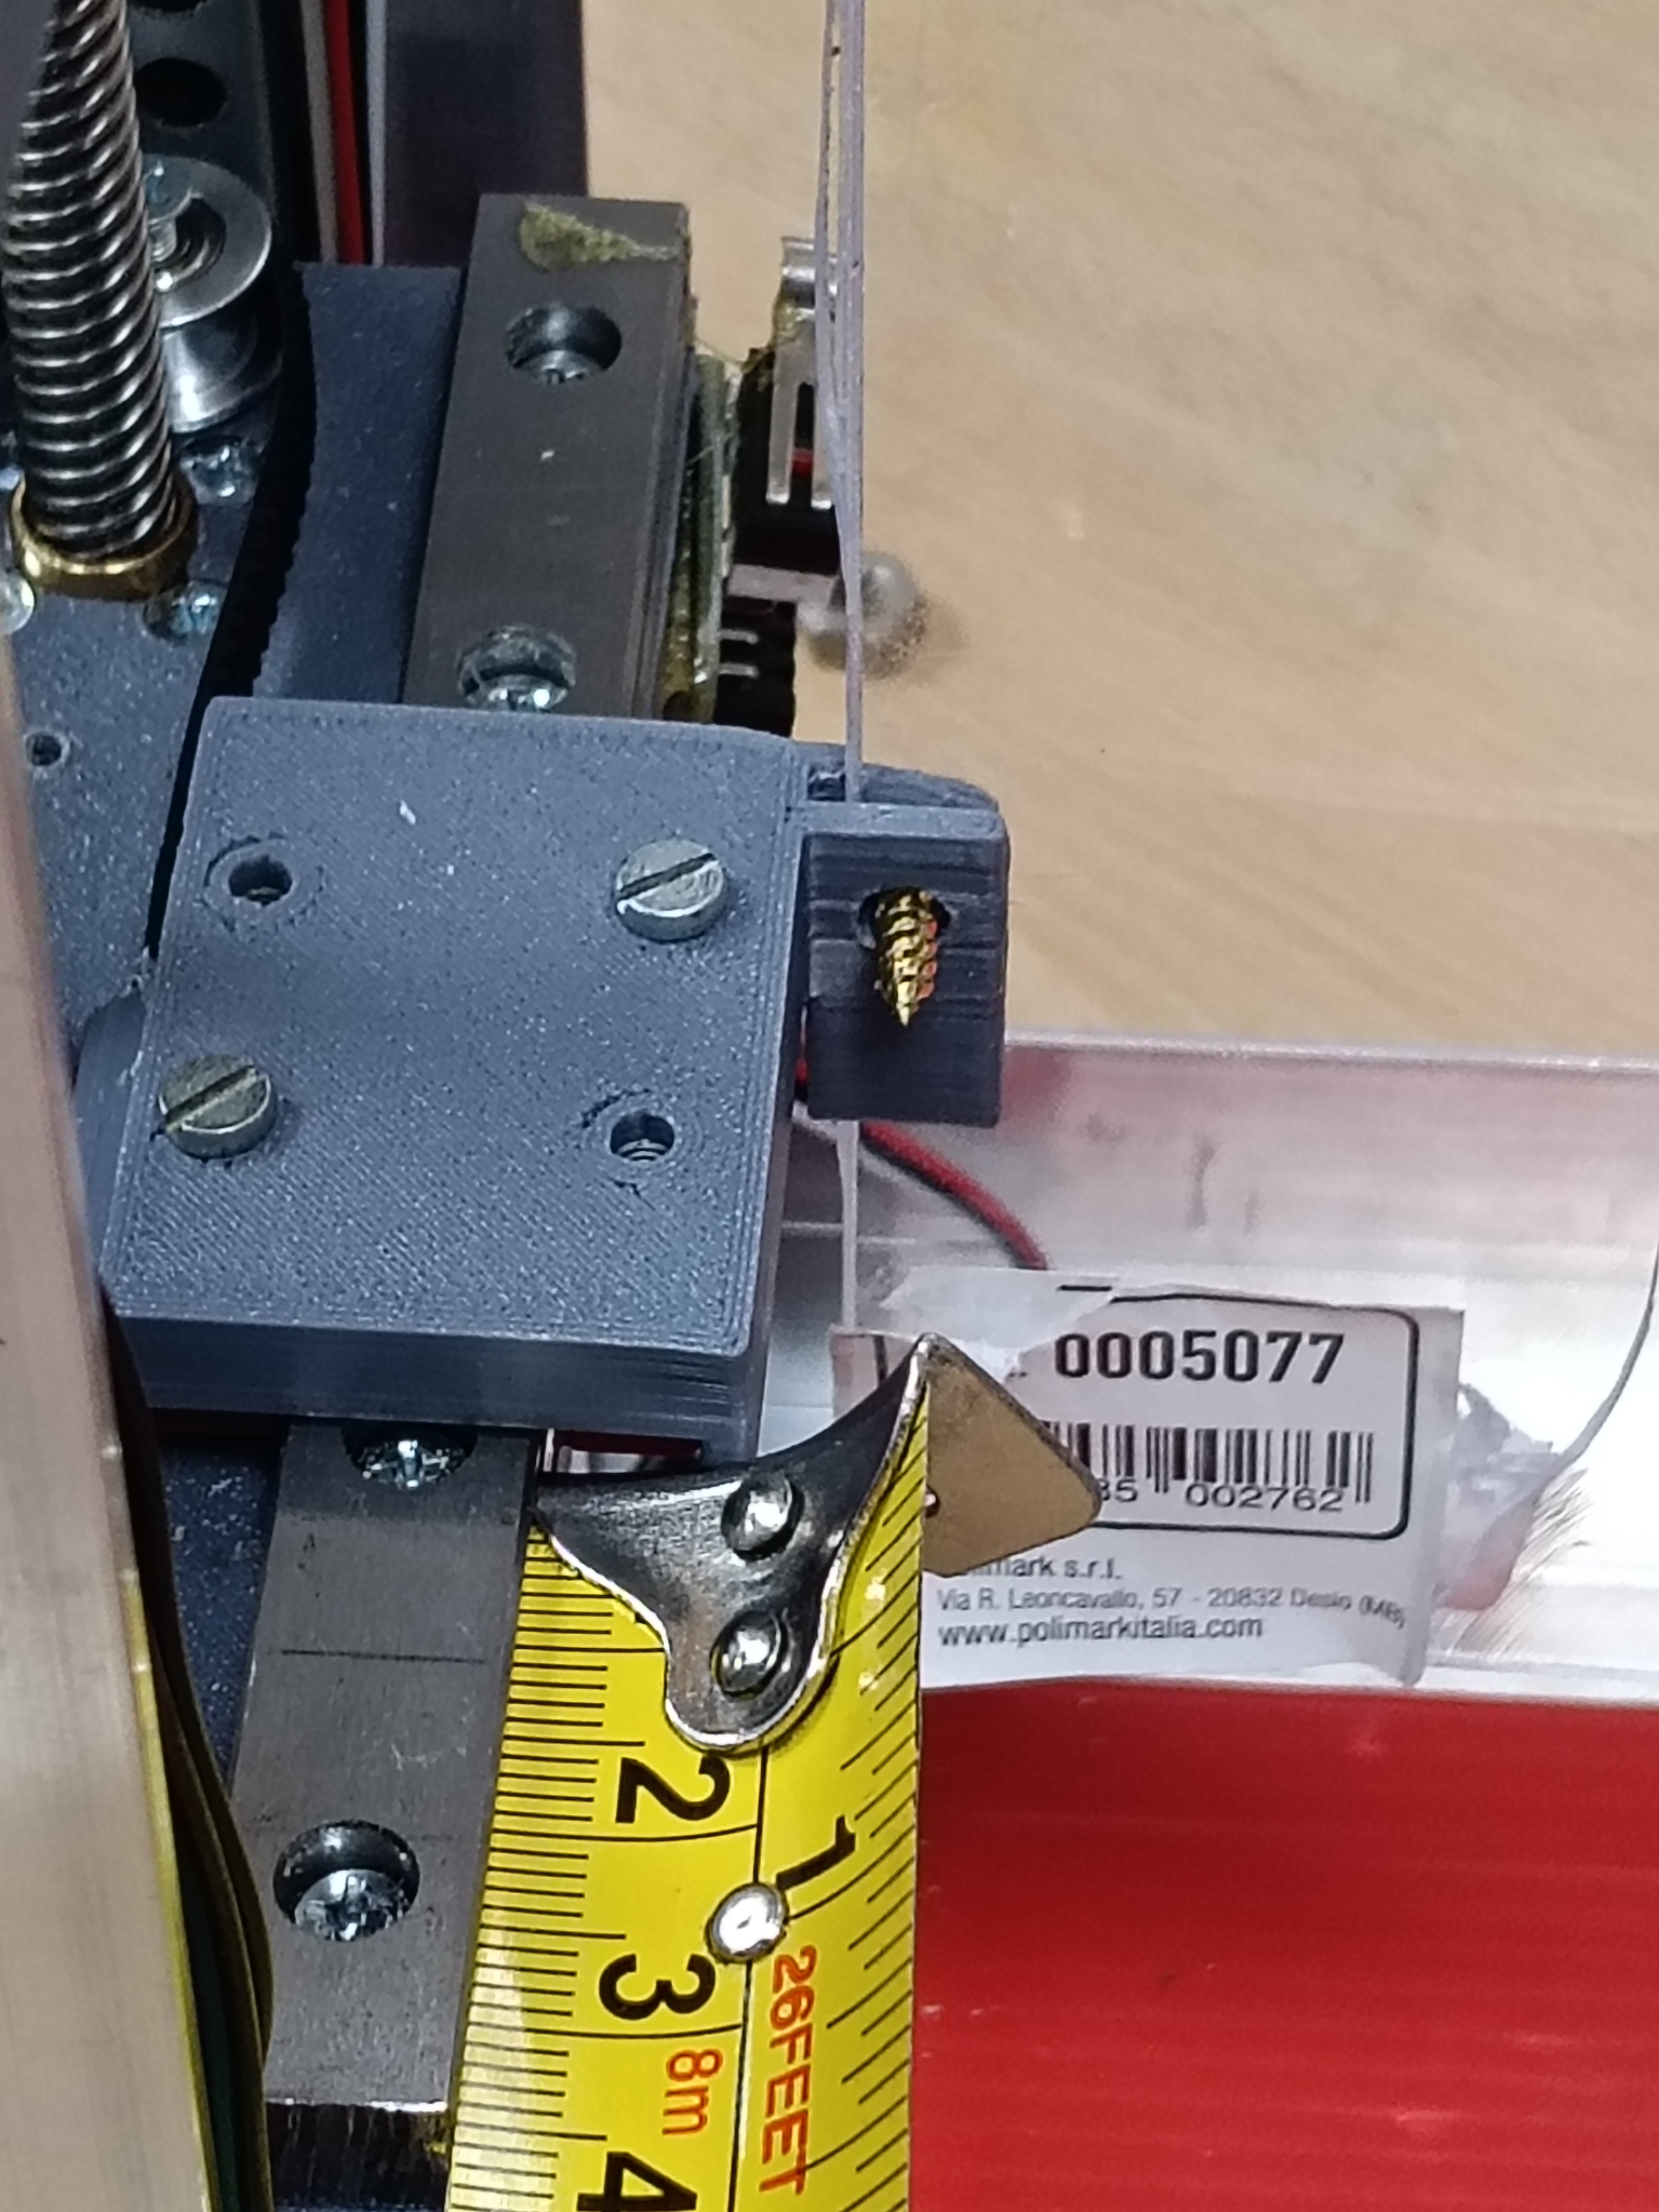
\includegraphics[width=0.45\linewidth]{figuras/pmmhb}
		}
		
		\caption*{\textbf{Caso A:} Movimiento a $X=50\,\mathrm{mm}$ y $Z=50\,\mathrm{mm}$.}
	\end{minipage}
	
	\vspace{1em}	
	
	% ===== PAREJA 3 =====
	\begin{minipage}{\linewidth}
		\centering
		\subfloat[$X_3 = 52 - 10 = 42\,\mathrm{mm}$]{
			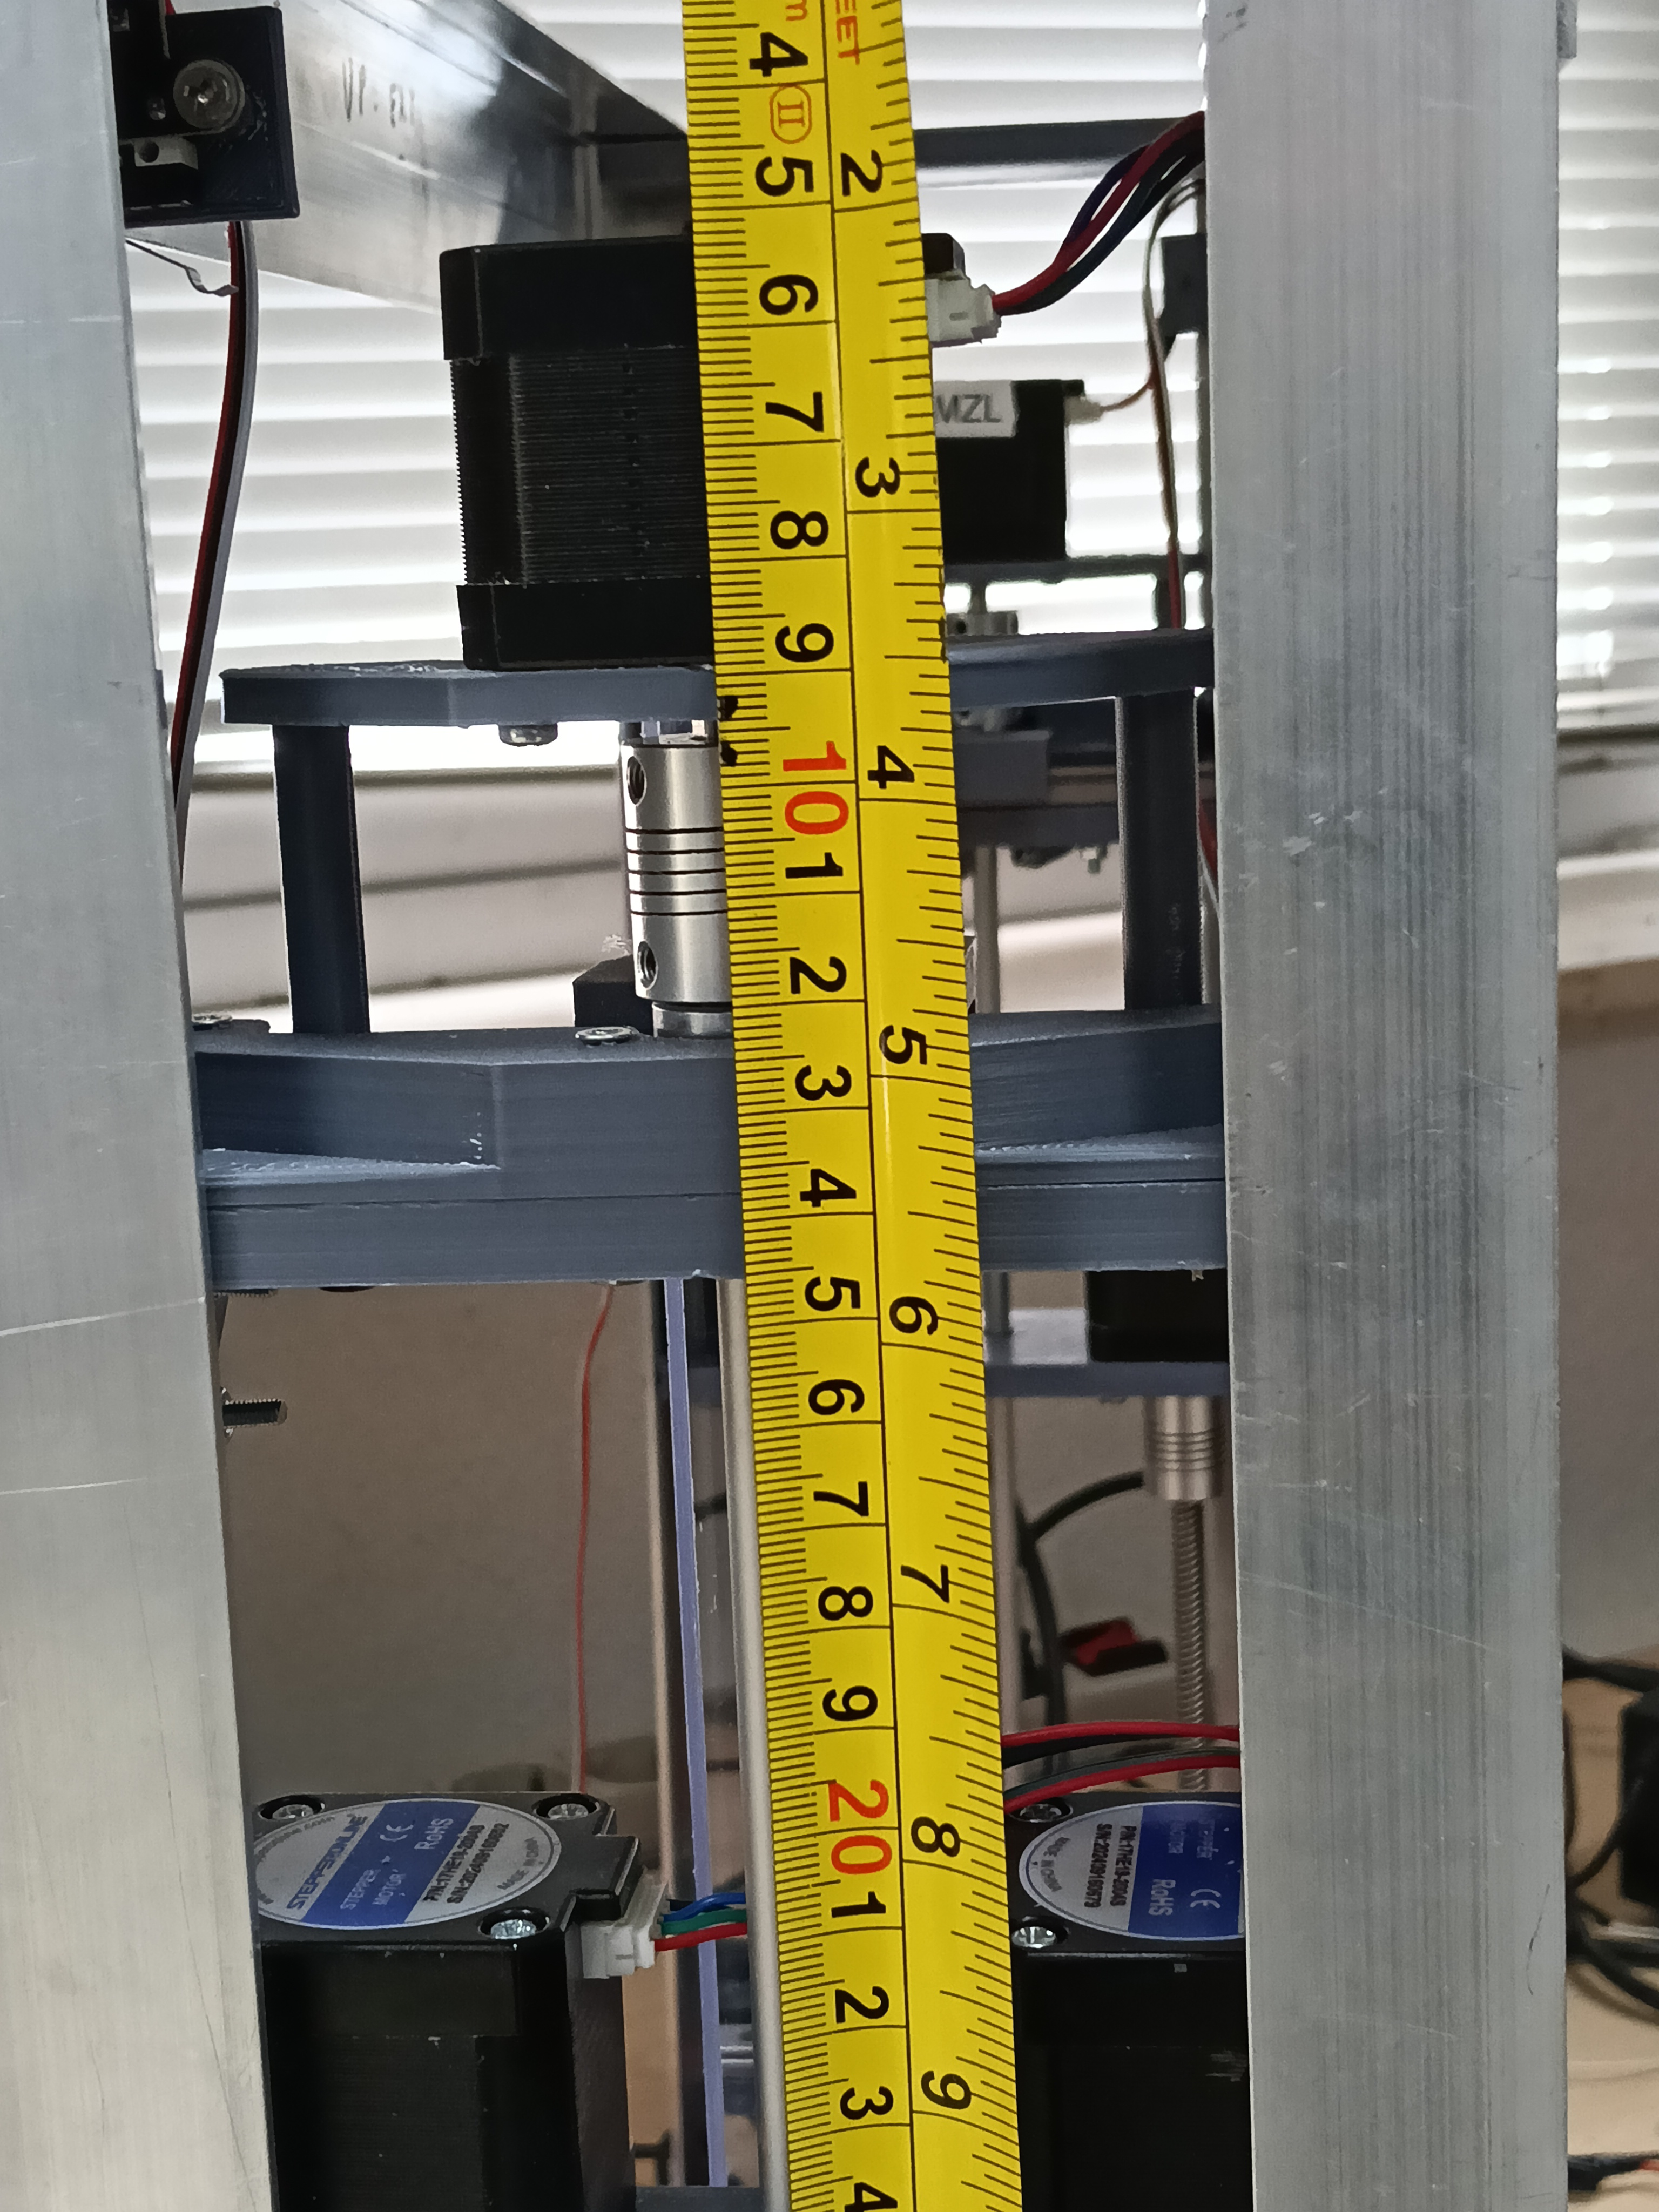
\includegraphics[width=0.45\linewidth]{figuras/pmmvc}
		}
		\subfloat[$Z_3 = 85 - 39 = 46\,\mathrm{mm}$]{
			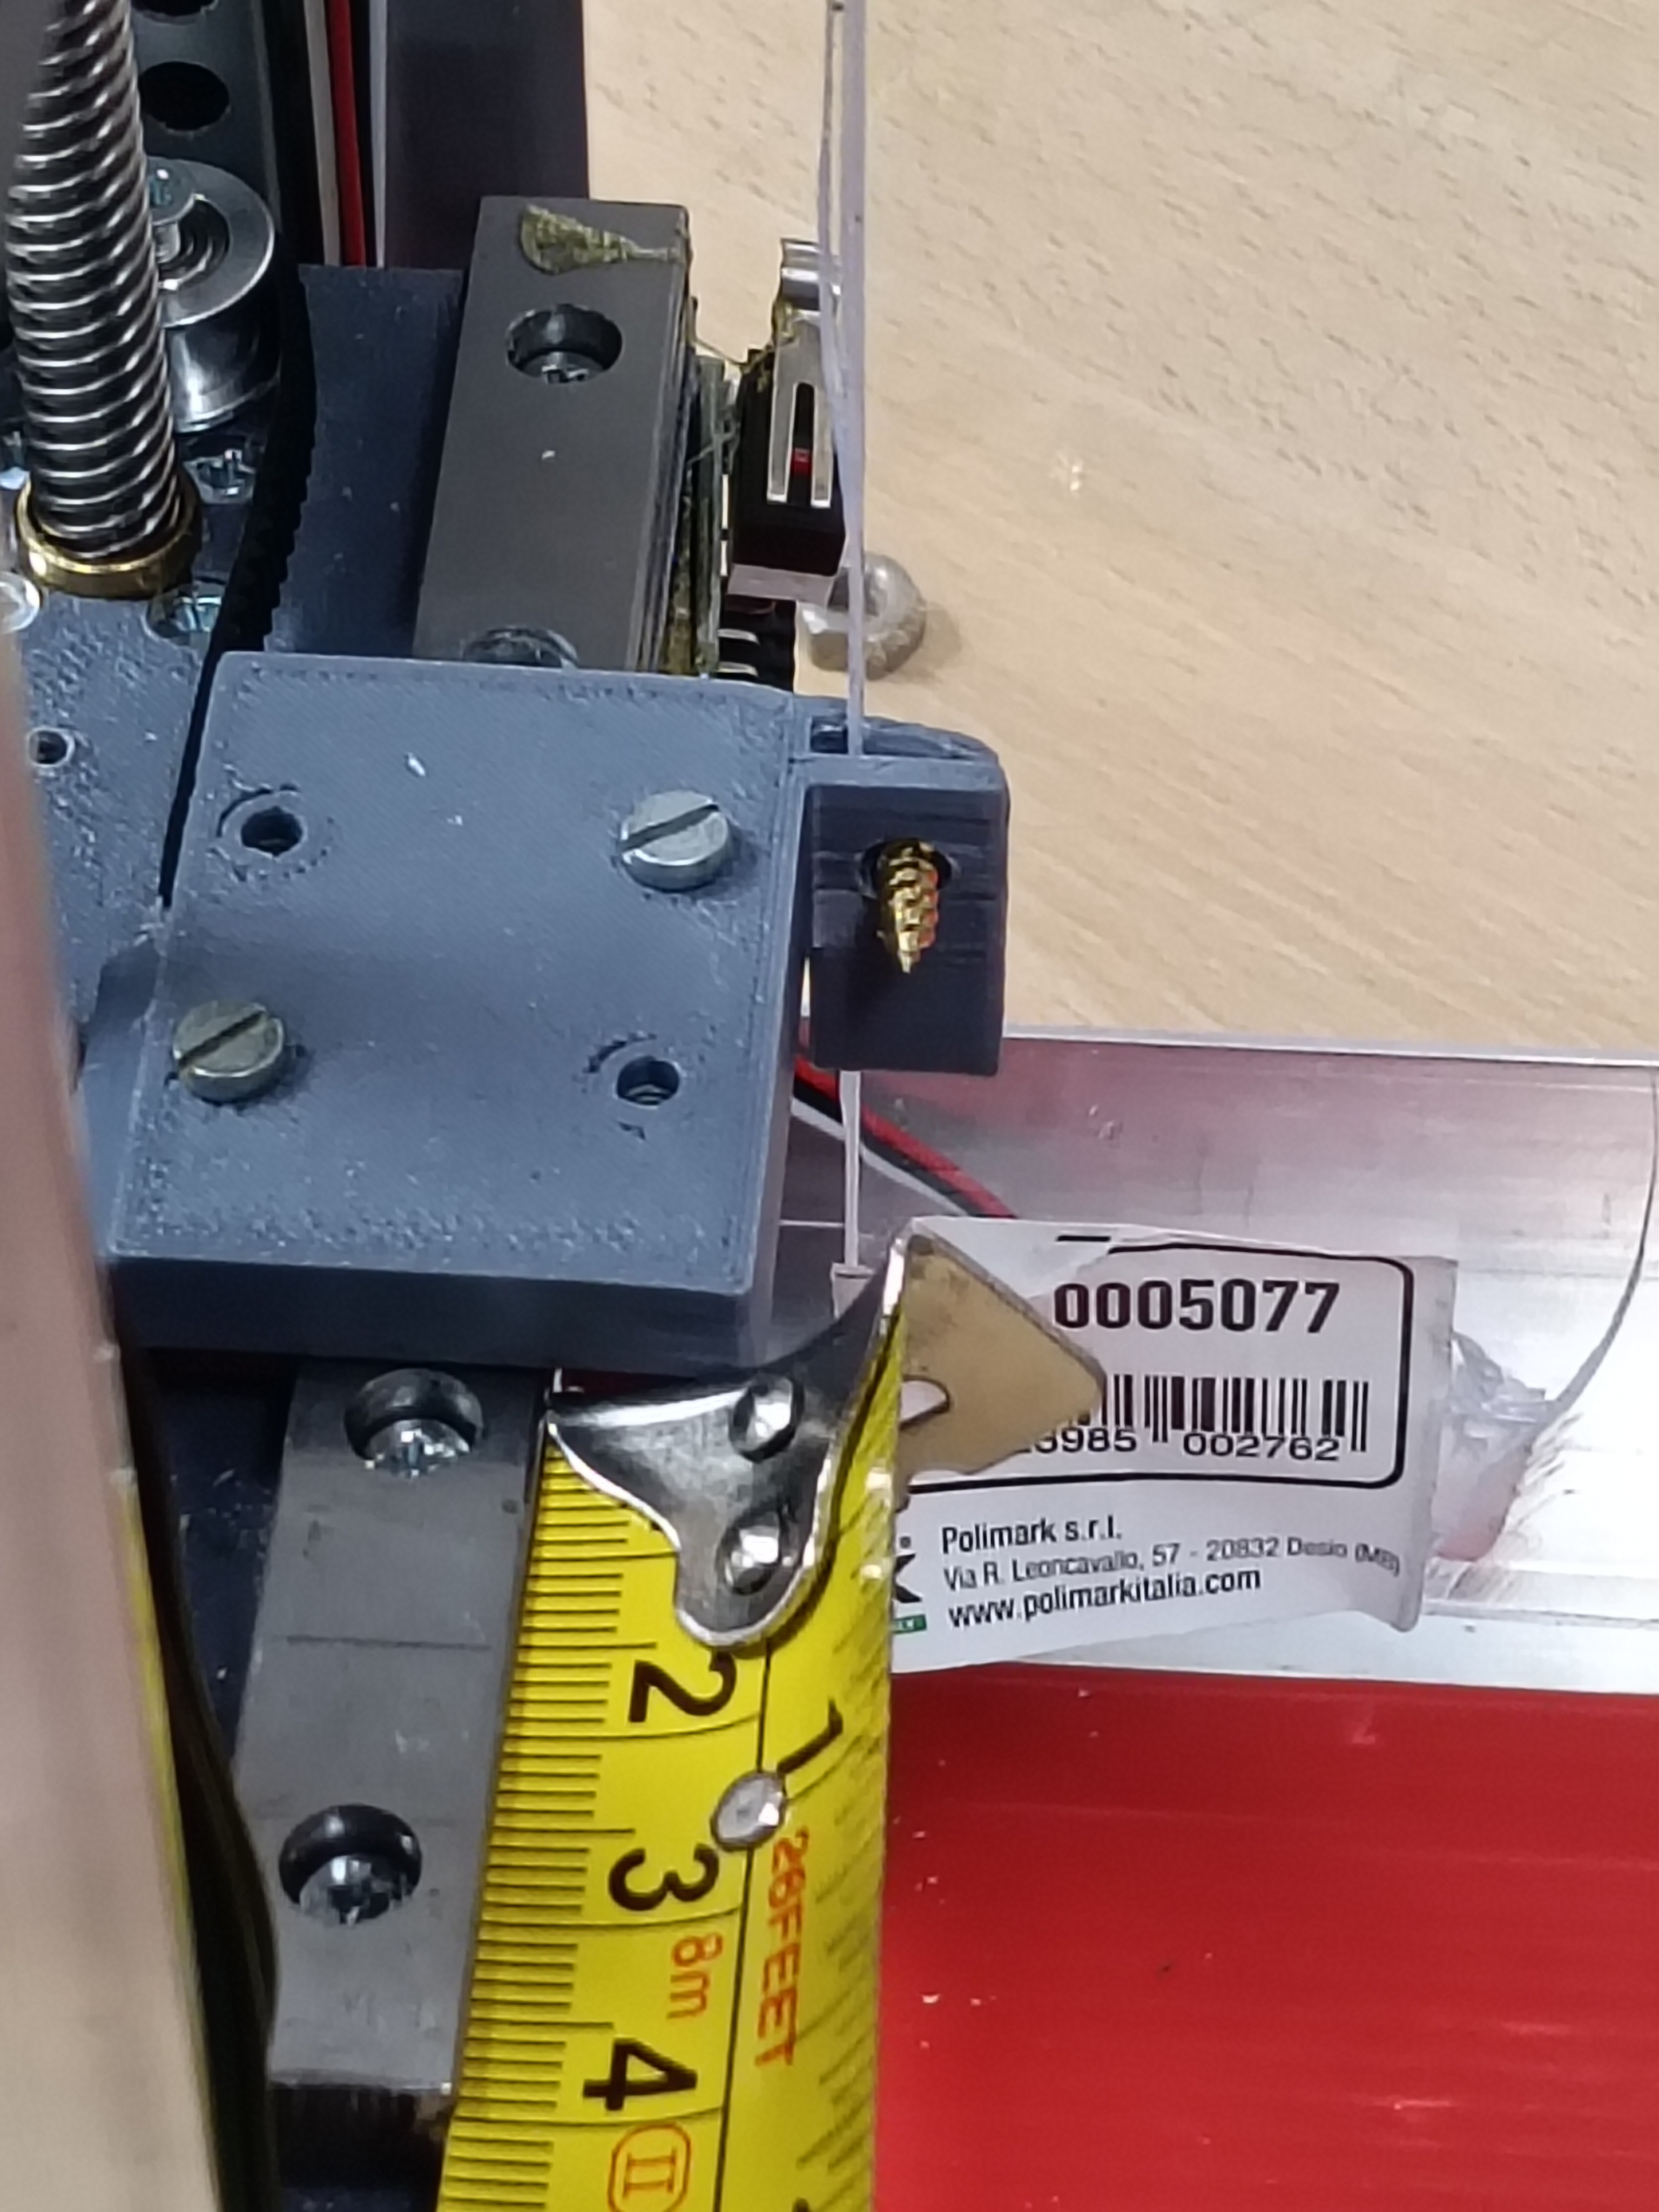
\includegraphics[width=0.45\linewidth]{figuras/pmmhc}
		}
		
		\caption*{\textbf{Caso B:} Movimiento a $X=42\,\mathrm{mm}$ y $Z=46\,\mathrm{mm}$.}
	\end{minipage}
\end{figure}

\begin{figure}	
	\centering
	\ContinuedFloat
	\subfloat[$X_1 = 35 - 10 = 25\,\mathrm{mm}$]{
		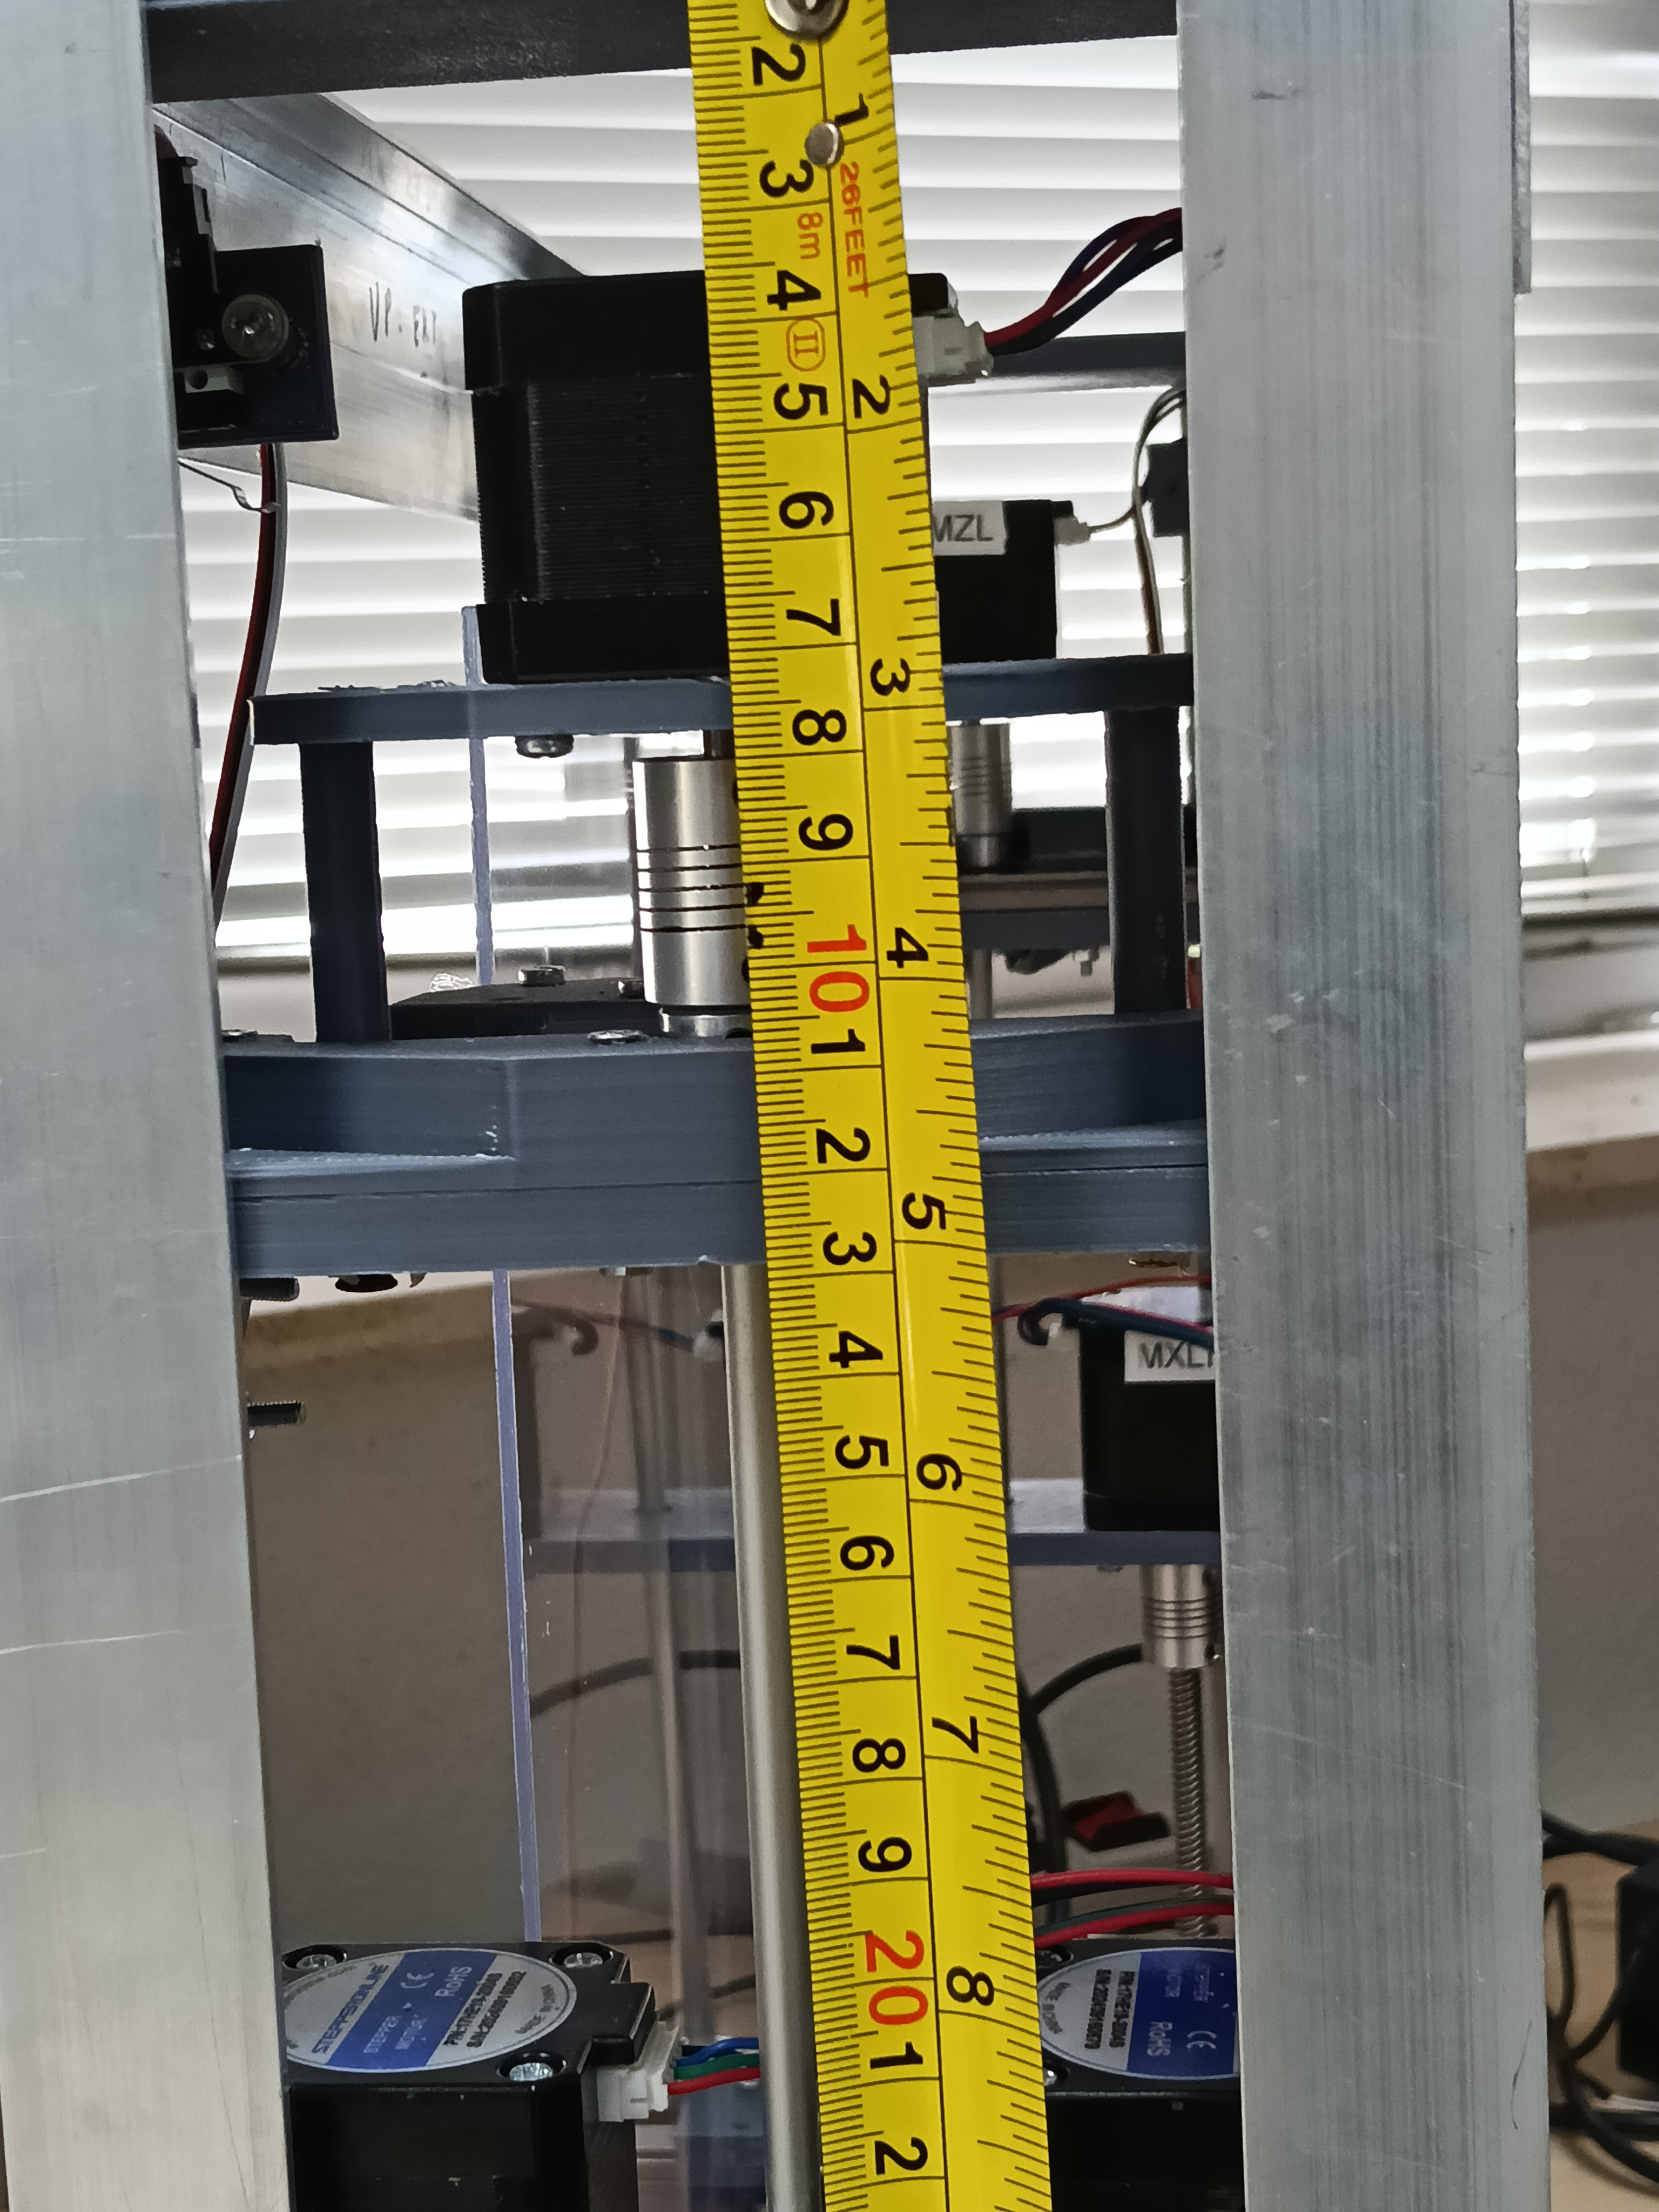
\includegraphics[width=0.45\linewidth]{figuras/pmmva}
	}	
	\subfloat[$Z_1 = 85 - 60 = 25\,\mathrm{mm}$]{
		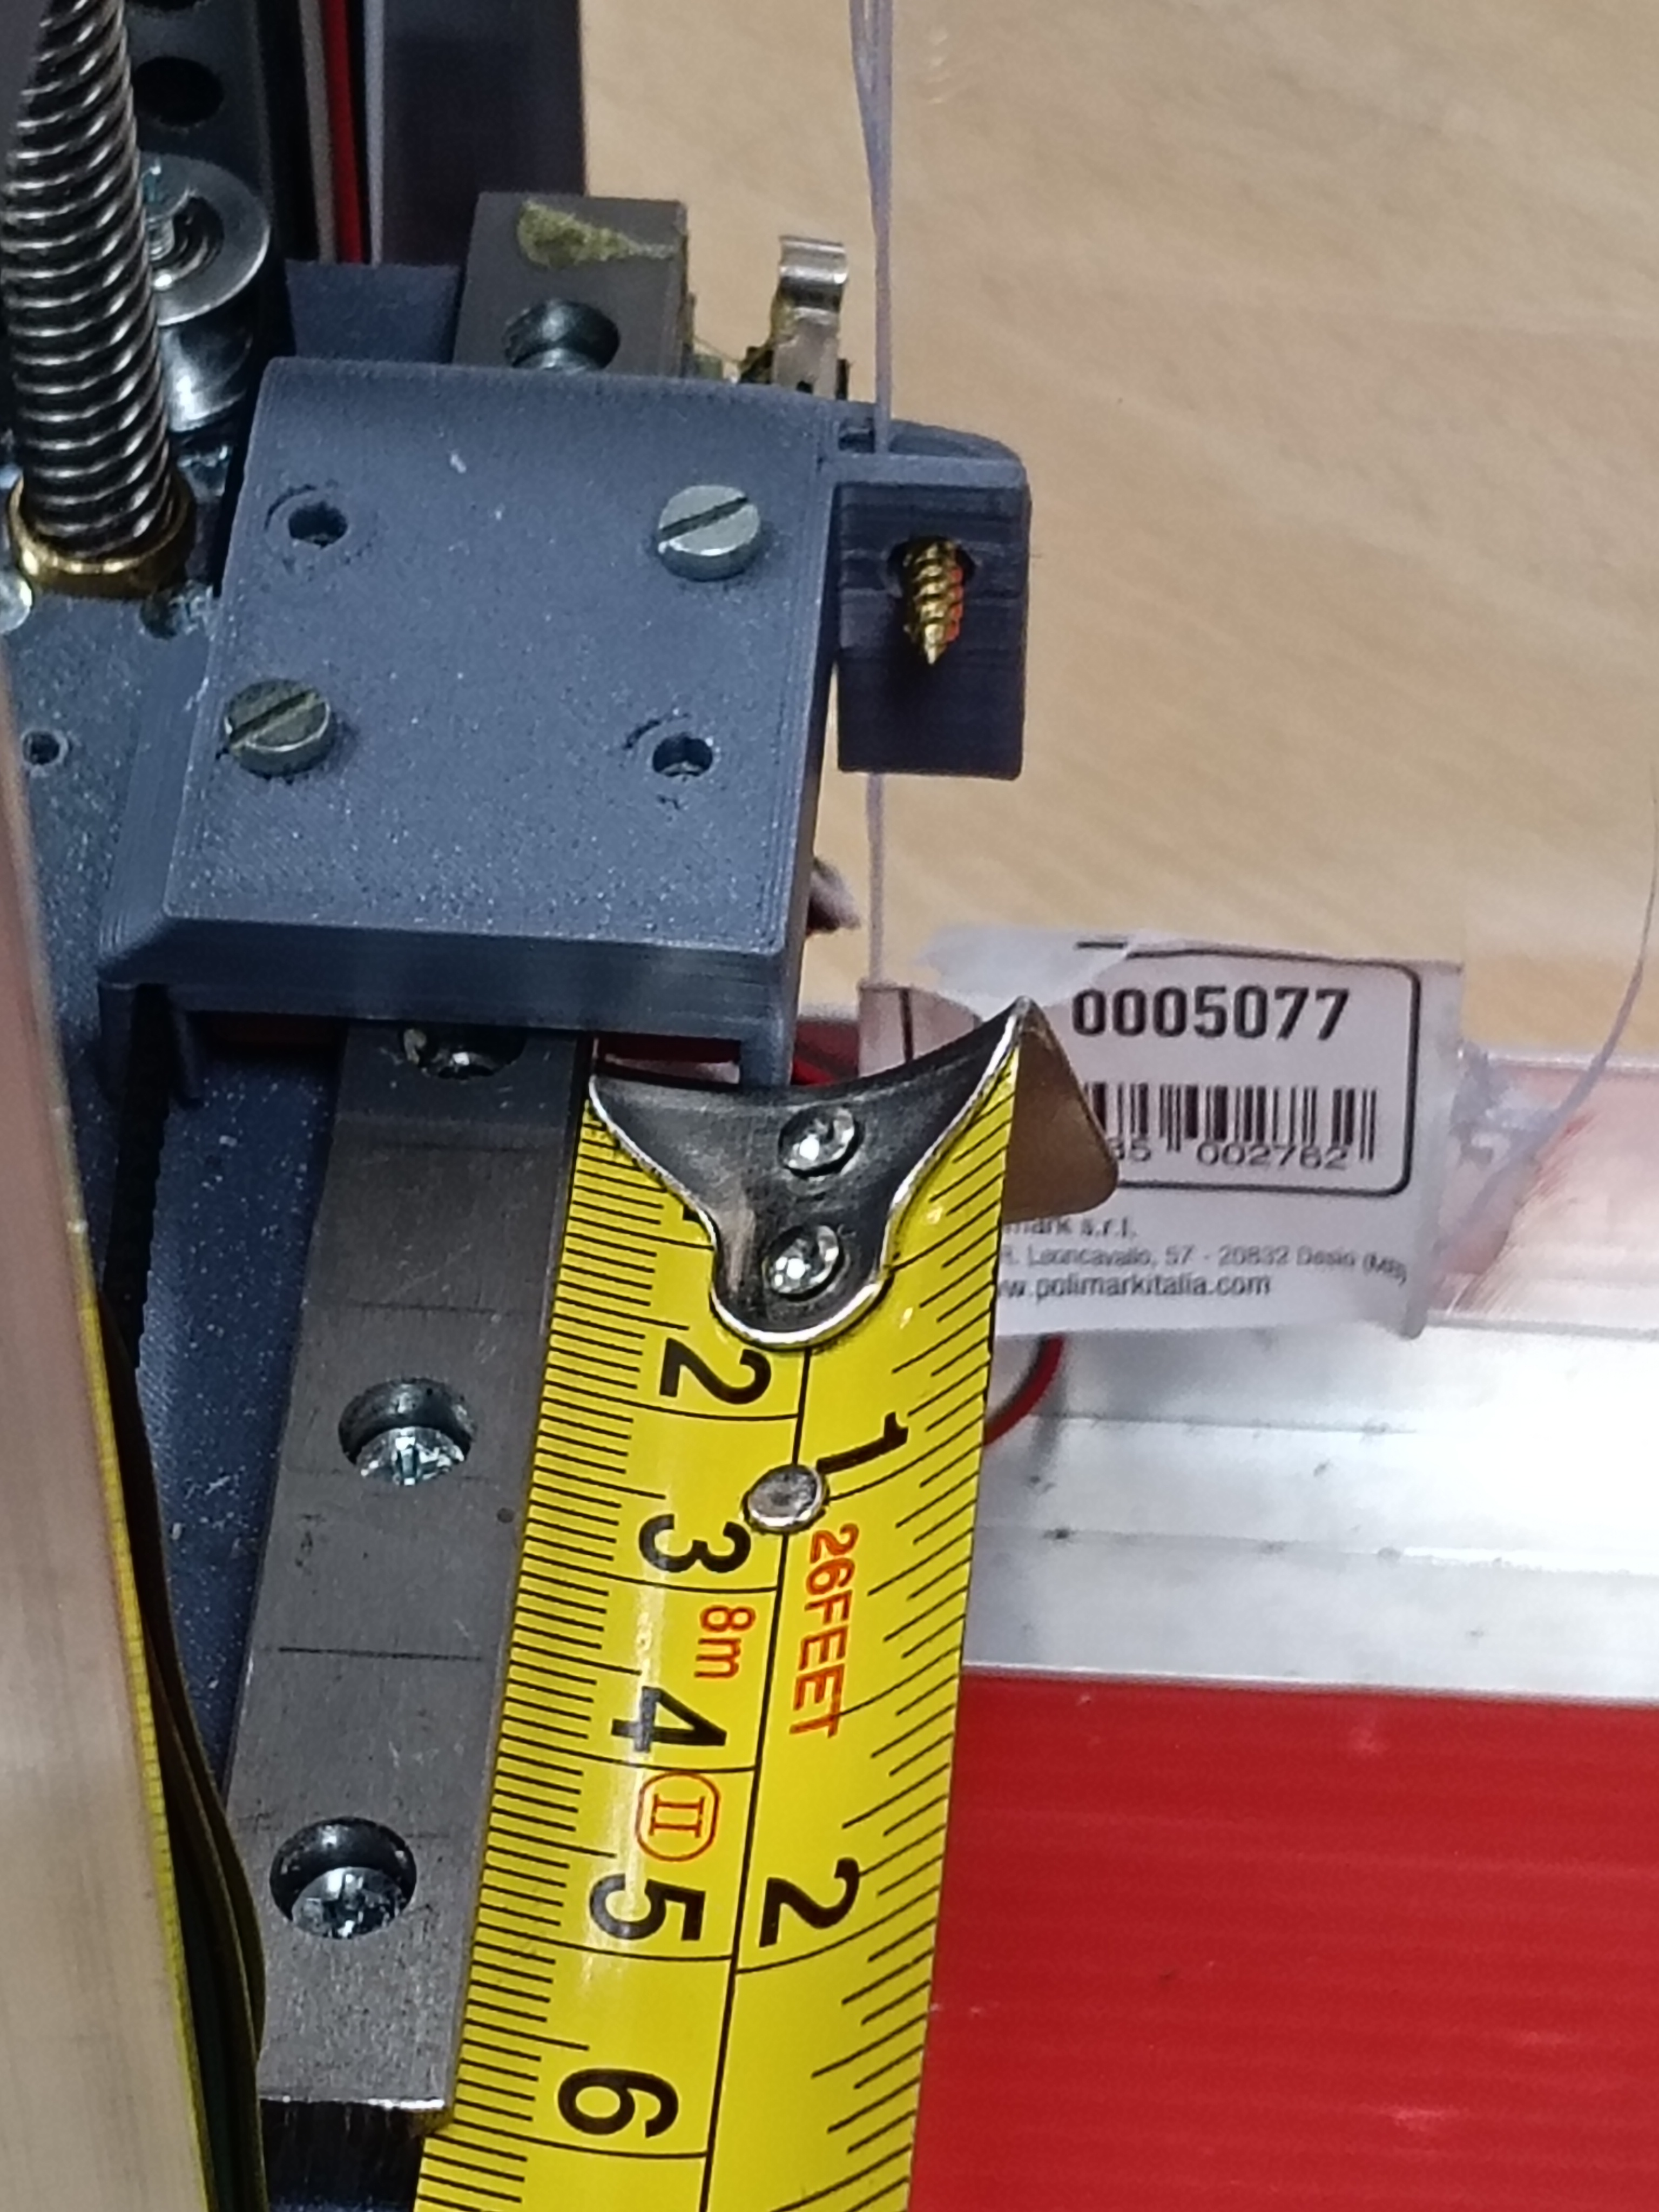
\includegraphics[width=0.45\linewidth]{figuras/pmmha}
	}
	
	\caption*{\textbf{Caso C:} Movimiento a $X=25\,\mathrm{mm}$ y $Z=25\,\mathrm{mm}$.}
	
\end{figure}

	

\section{Hojas de características}


\begin{figure}[t]
	\centering
	\subfloat[]{
		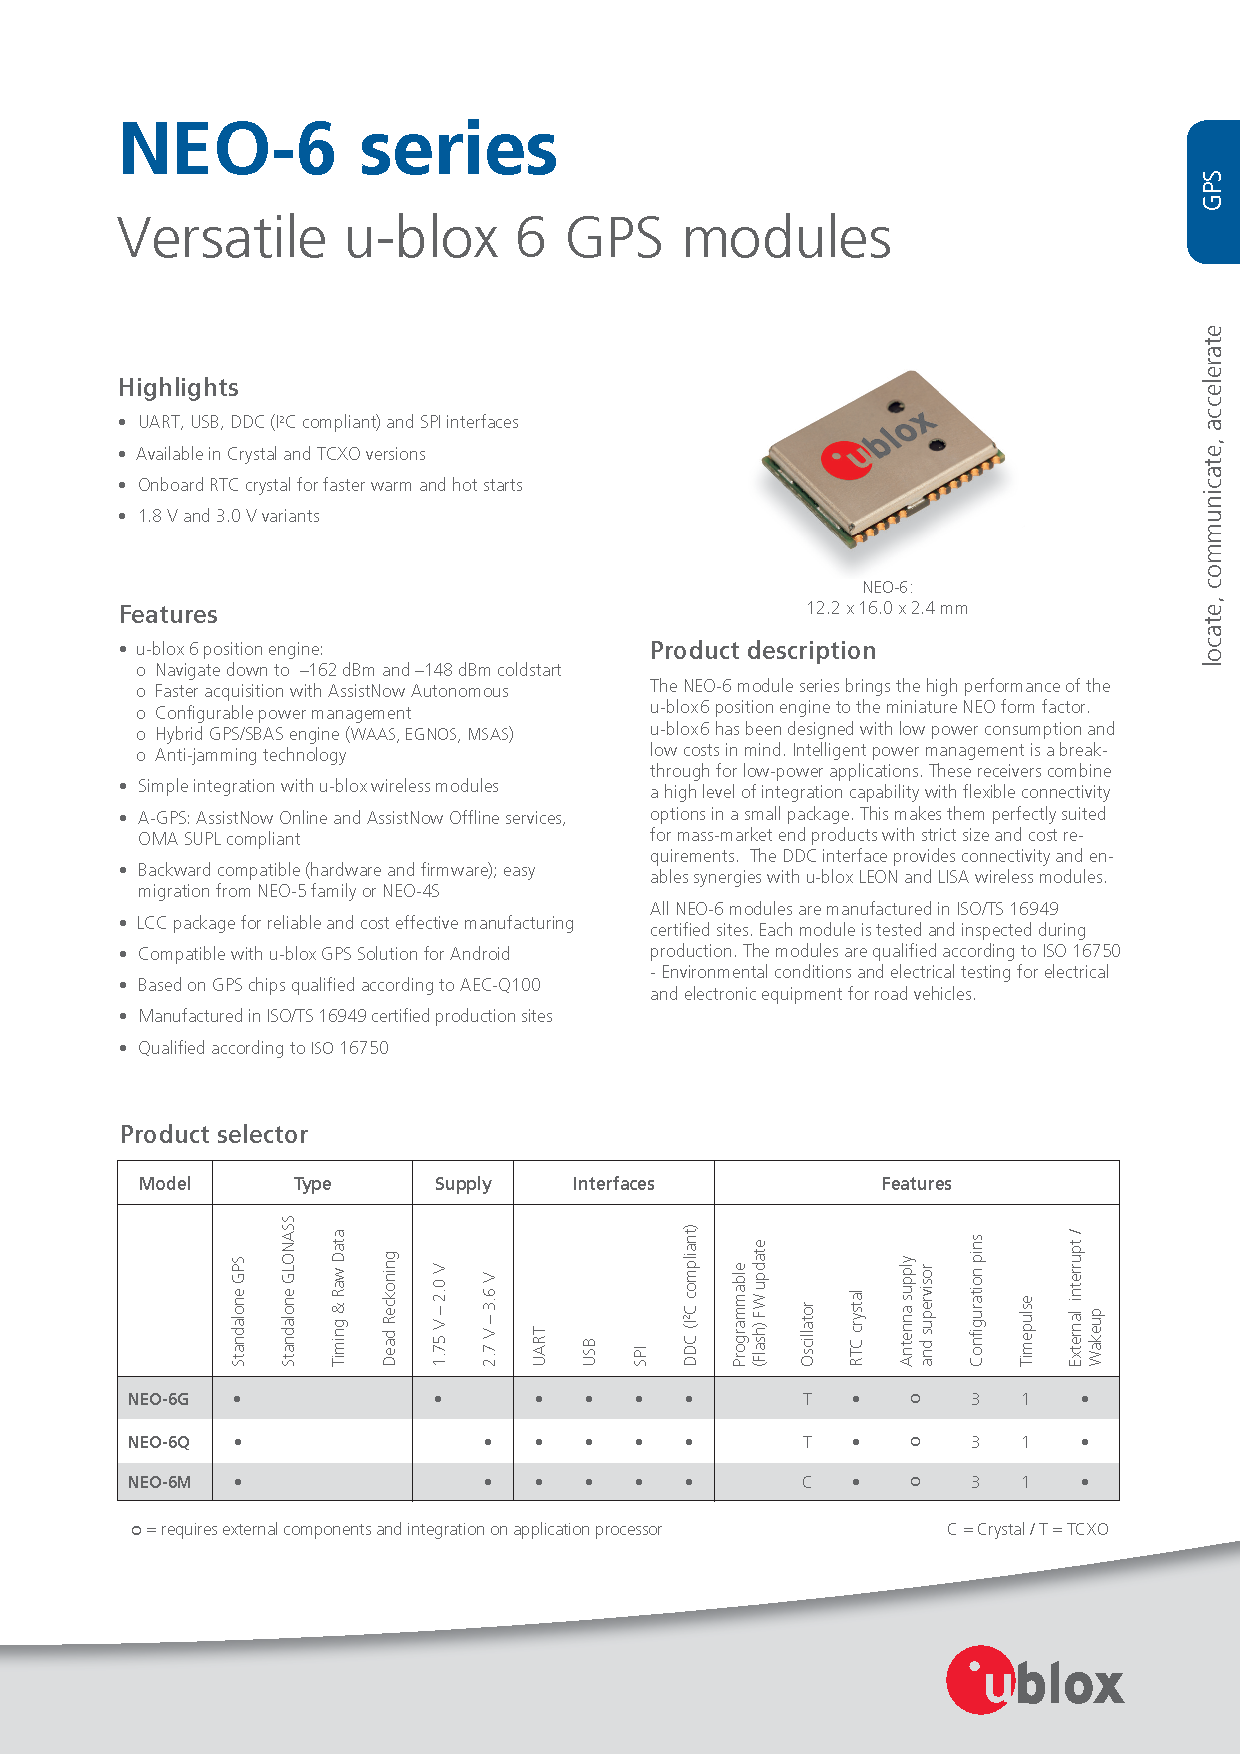
\includegraphics[width=0.99\linewidth, page=1]{figuras/datasheet_NEO-6}
	}
\end{figure}	

\begin{figure}
	\centering
	\ContinuedFloat	
	\subfloat[]{
		\includegraphics[width=0.99\linewidth, page=2]{figuras/datasheet_NEO-6}
	}
	\caption{Hoja de características del NEO-6M. Alldatasheet}
\end{figure}



\begin{figure}[t]
	\centering
	\subfloat[Nema-17]{
		\includesvg[width=0.99\linewidth]{figuras/data_nema17}
	}
	
	\subfloat[NEMA-17 42x42x38]{
		\includesvg[width=0.49\linewidth]{figuras/nema_pequeno}
	}
		\subfloat[NEMA-17 42x42x38]{
		\includesvg[width=0.49\linewidth]{figuras/nema_grande}
	}
	\caption{Hoja de características de los motores NEMA-17. Alldatasheet}
\end{figure}

 
 \begin{figure}[t]
 	\centering
 	\subfloat[Pinout.]{
 		\includesvg[width=0.99\linewidth]{figuras/cnc_datasheet}
 	}
 	

 	\subfloat[Esquemático.]{
 		\includesvg[width=0.99\linewidth]{figuras/cnc_shield_2}
 	}
 	\caption{Esquemáticos CNC-Shield-V3. Fuente: Alldatasheet}
 \end{figure}
 
 
 
 \begin{figure}[t]
 	\centering
 	\includesvg[width=0.69\linewidth]{figuras/daata_driver}
 	\caption{Esquemático driver A4998. Fuente: Amazon}
 \end{figure}
 
 \subsection{ESP32-S3-Devkit-C1}
 El enlace~\footnote{\url{https://documentation.espressif.com/esp32-s3-wroom-1_wroom-1u_datasheet_en.pdf}} accede a la hoja de características del módulo ESP32-S3 y la Figura~\ref{fig:esquematico_esp} contiene el esquemático de la placa de desarrollo Devkit-C1.
 
 \begin{figure}[t]
 	\centering
 	\subfloat[]{
 		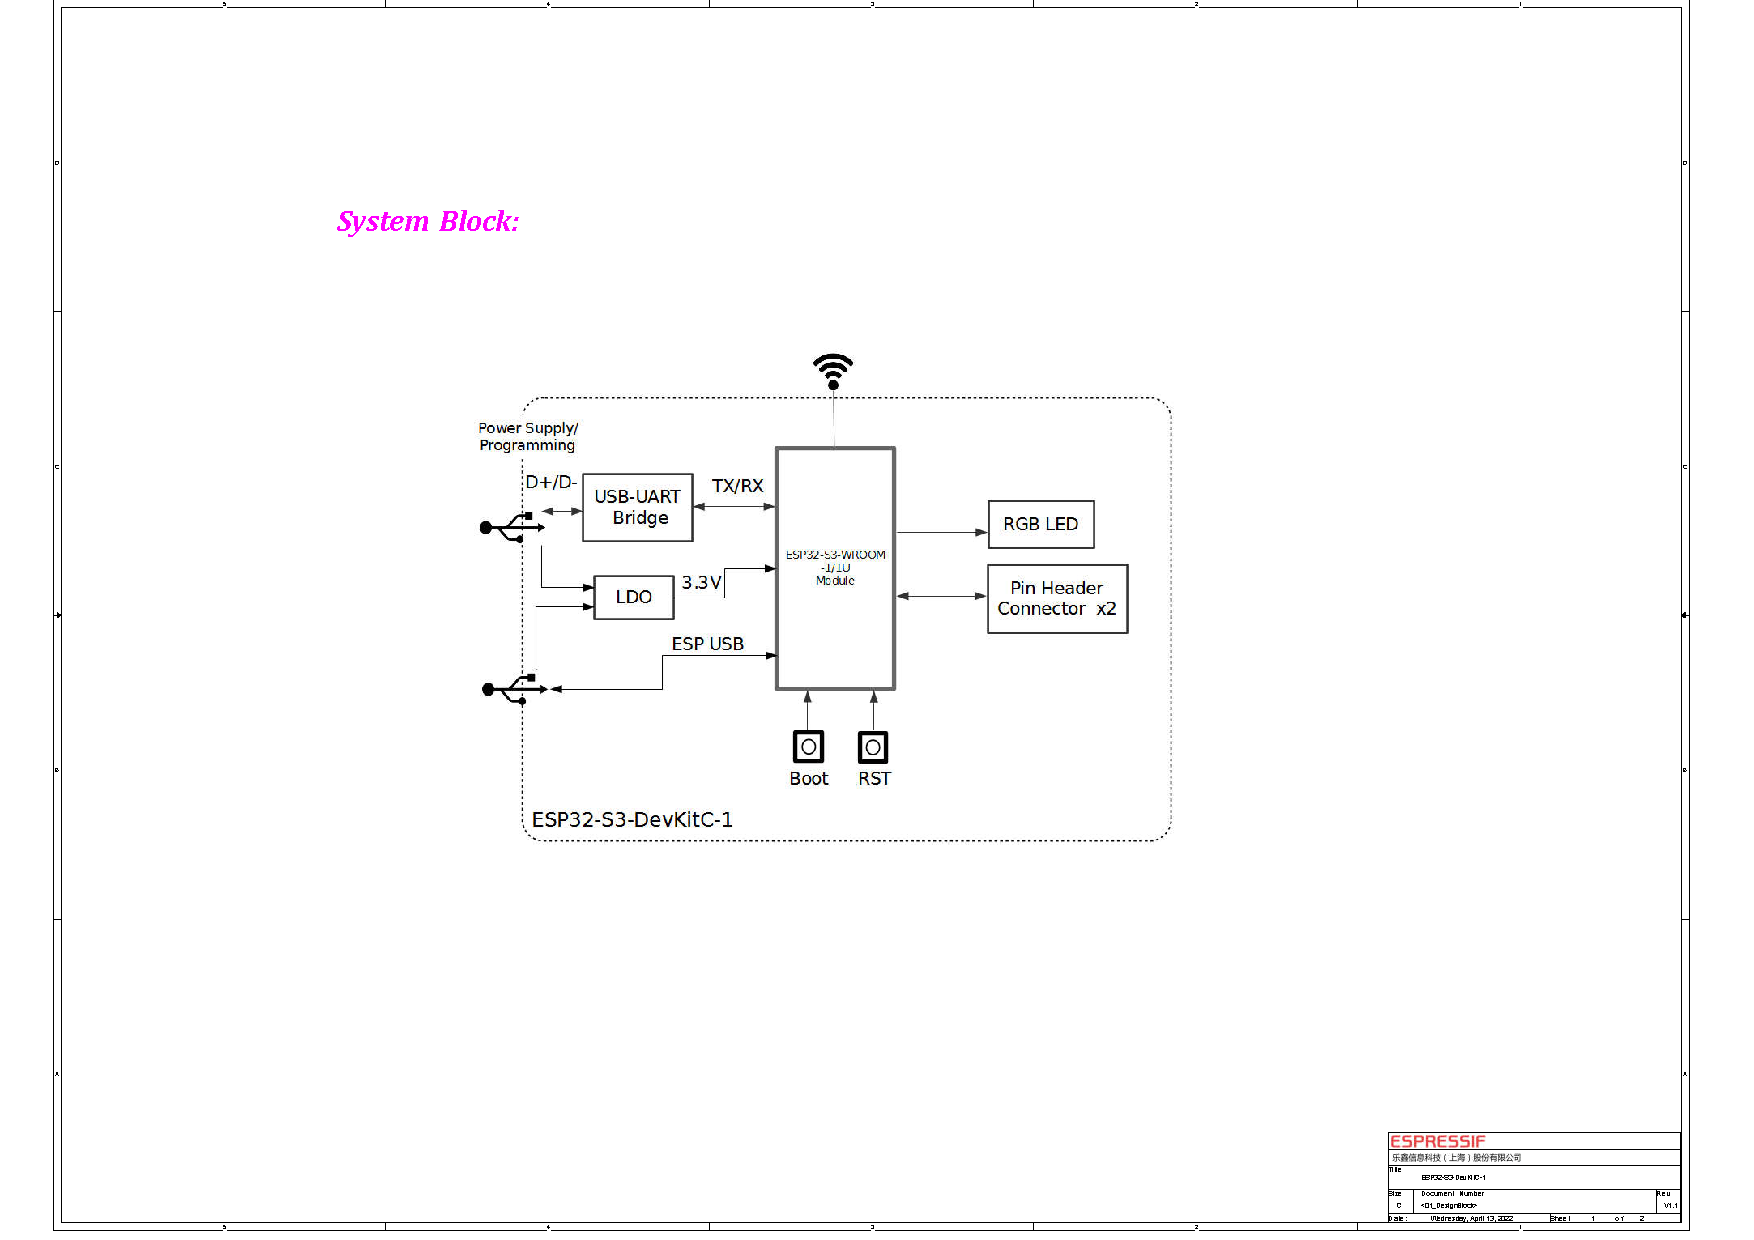
\includegraphics[width=0.99\linewidth, page=1]{figuras/SCH_ESP32-S3-DevKitC-1_V1.1_20221130}
 	}
 	
 	
 	\subfloat[]{
 		\includegraphics[width=0.99\linewidth, page=2]{figuras/SCH_ESP32-S3-DevKitC-1_V1.1_20221130}
 	}
 	\caption{Esquemático ESP32-S3-Devkit-C1. Alldatasheet}
 	\label{fig:esquematico_esp}
 \end{figure}
 